\documentclass{IEEEtran}
\usepackage[english]{babel}
\usepackage{caption}
\usepackage[export]{adjustbox}
%\usepackage{comment}
\usepackage{hyperref}
\usepackage{graphicx}
\usepackage{amsmath}
%\usepackage{authblk}
\graphicspath{{images/}}
\usepackage{geometry}
\usepackage{array}
\usepackage{color,soul}
\usepackage{tabularx}
 \geometry{
 a4paper,
 total={170mm,257mm},
 left=15mm,
 top=15mm,
 }
 \begin{document}
 \setcounter{page}{11}
 \begin{itemize}
 \item  \textbf{IOU accuracy of each class}
\begin{figure}[h]
    \centering
    \captionsetup{justification=centering}
    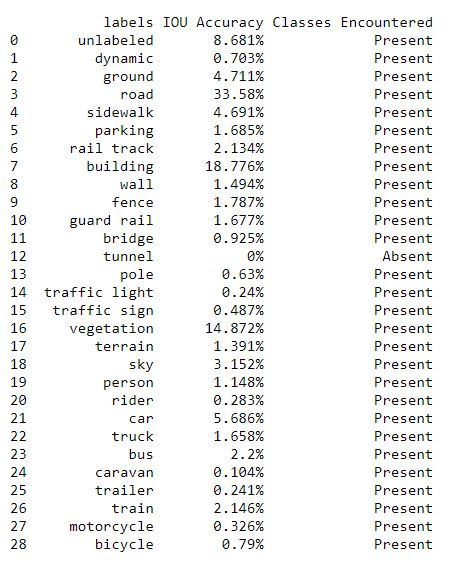
\includegraphics[width=7.5cm]{U-net-cityscrapes-B16-IOU-C29.JPG}
    \caption{U-net IOU per class}
    \label{fig:Binary class segmented output}
\end{figure}

\begin{figure}[h]
    \centering
    \captionsetup{justification=centering}
    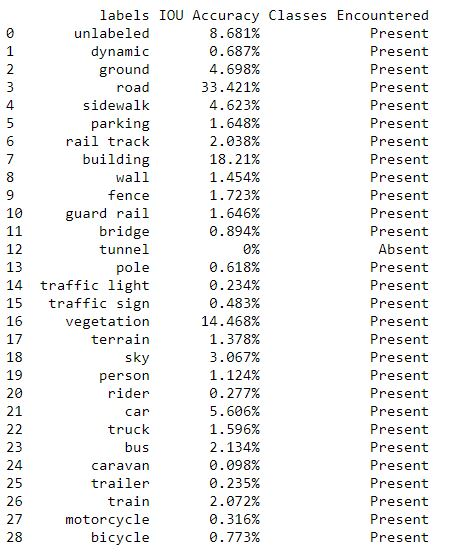
\includegraphics[width=7.5cm]{Segnet-cityscrapes-B16-IOU-C29.JPG}
    \caption{Segnet IOU per class}
    \label{fig:Binary class segmented output}
\end{figure}

\newpage

\begin{figure}[h]
    \centering
    \captionsetup{justification=centering}
    \includegraphics[width=7.5cm]{Resnet-cityscrapes-B16-IOU-C29.JPG}
    \caption{Resnet IOU per class}
    \label{fig:Binary class segmented output}
\end{figure}

\begin{figure}[h]
    \centering
    \captionsetup{justification=centering}
    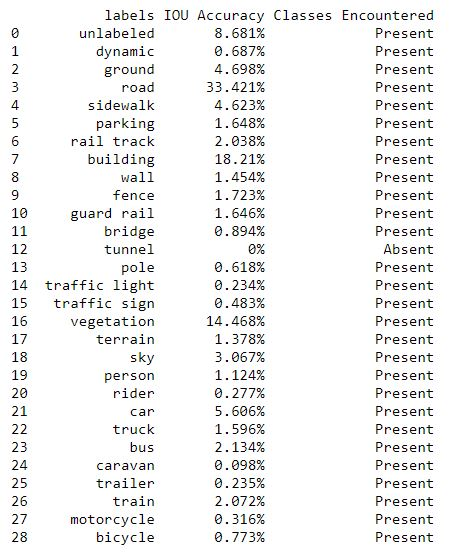
\includegraphics[width=7cm]{ICnet-cityscrapes-B16-IOU-C29.JPG}
    \caption{IC-net IOU per class}
    \label{fig:Binary class segmented output}
\end{figure}
\end{itemize}

In all the architectures, class road was detected most accurately.\\
1. U-net : 91.998\% \\
2. Segnet : 89.082\% \\
3. IC-net : 68.287\% \\
4. Resnet : 33.421\% \\
\newpage

\begin{center}
\textbf{XI AMAZON WEB SERVICES}    
\end{center}

Amazon web services was used to train the deep neural net models as powerful GPUs were required to perform convolution operation on big dataset like cityscrapes. The dataset was uploaded to Amazon cloud storage service called S3 bucket. Then, using one of the service of AWS called Sagemaker jupyter notebook was launched. The dataset stored on the S3 bucket storage device was made public in order to access the dataset from Sagemaker. The below diagram shows how to dataset is handled:

\begin{figure}[h]
    \centering
    \captionsetup{justification=centering}
    \includegraphics[width=8.5cm]{aws.JPG}
    \caption{Accesing the dataset from cloud}
    \label{fig:Binary class segmented output}
\end{figure}

AWS does not give GPU capabilities to its user by default. Therefore, GPU request need to be sent by the user to the AWS service explaining the need for the GPU. The above mentioned process was followed and the following GPU was allocated:
\begin{enumerate}
    \item GPU name : Tesla 1xK80
    \item Instance type: ml.p2.x.large instance
    \item number of vCPUs : 4
    \item RAM : 61 GB
    \item GPU Memory: 12 GB
\end{enumerate}

\begin{center}
\textbf{XII CONCLUSION}    
\end{center}
An in depth study of convolutional neural networks used for semantic segmentation is obtained. Different CNN architectures like U-net, Segnet, Resnet and IC-net have been studied and implemented and the results have been compared. By comparing the results, it is clear that U-net performs better than other architectures with a MIOU accuracy of 53.29\%. The reason U-net performs better is because in its expansion path, the concatenation of high resolution images from the contraction takes place. This restores the features lost during the upconvolution operation. Hence, it is recommended to use U-net for multiclass semantic segmentation.

\begin{center}
\textbf{XIII ARCHITECTURE SPEED COMPARISON}
\end{center}
Architecture speed here refers to the speed at which an architecture can perform semantic segmentation on an image and provide segmented output. In certain real life scenarios, speed matters more than accuracy of the architectures. The following table illustrates the speed of architectures in increasing order:
\\

\begin{tabular}{ |p{0.6cm}|p{1.8cm}|p{4cm}|}
 \hline
 \multicolumn{3}{|c|}{\textbf{Architecture Speed Results}} \\
 \hline
 \textbf{Sno} & \textbf{Architecture} & \textbf{Average speed per sample}\\
 \hline
 1. & Resnet34   & 45.42 milli seconds \\
 \hline
 2. & IC-net   & 45.5 milli seconds  \\
 \hline
 3. & U-net   & 121.54 milli seconds   \\
 \hline
 4. & Segnet   & 128.615 milli seconds  \\
 \hline
\end{tabular}
\\
\\
From the table, it can be inferred that Resnet34 architecture performs semantic segmentation quickly than U-net, Segnet and IC-net

\begin{center}
\textbf{XIV REFERENCES}    
\end{center}
\begin{enumerate}
\item Layers of a Convolutional Neural Network. (2020, March 02). Retrieved from https://mc.ai/layers-of-a-convolutional-neural-network/

\item MACMAC 51644 silver badges1414 bronze badges. (1969, October 01). Understanding Gaussian Filter and how to plot it in 1-D. Retrieved from https://stackoverflow.com/questions/60462388/understanding-gaussian-filter-and-how-to-plot-it-in-1-d

\item Anh H. Reynolds. (2017, October 15). Convolutional Neural Networks (CNNs). Retrieved from https://anhreynolds.com/blogs/cnn.html

\item Diterbitkan oleh Benny Prijono Lihat semua pos dari Benny Prijono, Prijono, D., Prijono, B., Lihat semua pos dari Benny Prijono, 14, P., Berkata:, P., . . . (wajib), N. (2018, April 03). Student Notes: Convolutional Neural Networks (CNN) Introduction. Retrieved June 26, 2020, from https://indoml.com/2018/03/07/student-notes-convolutional-neural-networks-cnn-introduction/

\item Sakshi TiwariCheck out this Author's contributed articles., Sakshi Tiwari, amp; Check out this Author's contributed articles. (2018, February 06). Activation functions in Neural Networks. Retrieved June 26, 2020, from https://www.geeksforgeeks.org/activation-functions-neural-networks/

\item Intro to Linear vs. Nonlinear Functions. (n.d.). Retrieved June 26, 2020, from https://www.expii.com/t/intro-to-linear-vs-nonlinear-functions-4318

\item V, A. (2017, March 30). Understanding Activation Functions in Neural Networks. Retrieved July 02, 2020, from https://medium.com/the-theory-of-everything/understanding-activation-functions-in-neural-networks-9491262884e0

\item KIDS, T. (2019, July 31). Fully-Connected Layer with dynamic input shape. Retrieved July 03, 2020, from https://medium.com/@tecokids.monastir/fully-connected-layer-with-dynamic-input-shape-70c869ae71af

\item Singh, S. (2019, March 02). Fully Connected Layer: The brute force layer of a Machine Learning model. Retrieved July 03, 2020, from https://iq.opengenus.org/fully-connected-layer/

\item Uniqtech. (2020, April 21). Understand the Softmax Function in Minutes. Retrieved July 03, 2020, from https://medium.com/data-science-bootcamp/understand-the-softmax-function-in-minutes-f3a59641e86d

\item (PDF) A Deep Feature Learning Method for Drill Bits Monitoring Using the Spectral Analysis of the Acoustic Signals. (n.d.). Retrieved July 03, 2020, from https://www.researchgate.net/publication/327007086 A Deep Feature Learning Method for Drill Bits Monitoring Using the Spectral Analysis of the Acoustic Signals

\item Daniil's blog. (n.d.). Retrieved July 03, 2020, from http://warmspringwinds.github.io/tensorflow/tf-slim/2016/11/22/upsampling-and-image-segmentation-with-tensorflow-and-tf-slim/

\item 2018 Data Science Bowl. (n.d.). Retrieved July 06, 2020, from https://www.kaggle.com/c/data-science-bowl-2018/data

\item Jcoral. (2019, August 25). CamVid. Retrieved July 06, 2020, from https://www.kaggle.com/jcoral02/camvid

\item Badrinarayanan, Vijay, et al. “SegNet: A Deep Convolutional Encoder-Decoder Architecture for Image Segmentation.” ArXiv.org, 10 Oct. 2016, arxiv.org/abs/1511.00561.

\item Profile, bdd-data.berkeley.edu/portal.html.

\item Ronneberger, O., Fischer, P.; Brox, T. (2015, May 18). U-Net: Convolutional Networks for Biomedical Image Segmentation. Retrieved August 20, 2020, from https://arxiv.org/abs/1505.04597

\item Zhao, H., Qi, X., Shen, X., Shi, J.; Jia, J. (2018, August 20). ICNet for Real-Time Semantic Segmentation on High-Resolution Images. Retrieved August 20, 2020, from https://arxiv.org/abs/1704.08545

\item He, K., Zhang, X., Ren, S.,; Sun, J. (2015, December 10). Deep Residual Learning for Image Recognition. Retrieved August 20, 2020, from https://arxiv.org/abs/1512.03385

\item Zhang, X., Zou, J., He, K., ; Sun, J. (2015, November 18). Accelerating Very Deep Convolutional Networks for Classification and Detection. Retrieved from https://arxiv.org/abs/1505.06798

\item Zhao, H., Shi, J., Qi, X., Wang, X., ; Jia, J. (2017, April 27). Pyramid Scene Parsing Network. Retrieved August 23, 2020, from https://arxiv.org/abs/1612.01105
\end{enumerate}
 \end{document}